\subsection{Экспериментальная установка на пучковых тестах}\label{section:secBeamtimeSetup}

Исследование системы считывания и сбора данных проводилось в составе полнофункционального прототипа детектора RICH эксперимента CBM в ходе комплексных пучковых испытаний прототипов нескольких детекторов того же эксперимента~\cite{BEAMTIME}. Подробности реализации прототипов детектора переходного излучения и время-пролетного детектора содержатся в работах~\cite{TRDBEAMTIME}~и~\cite{TOFBEAMTIME} соответственно. Схема установки представлена на \figref{fig:Beamtime}.

\begin{figure}[H]
\centering
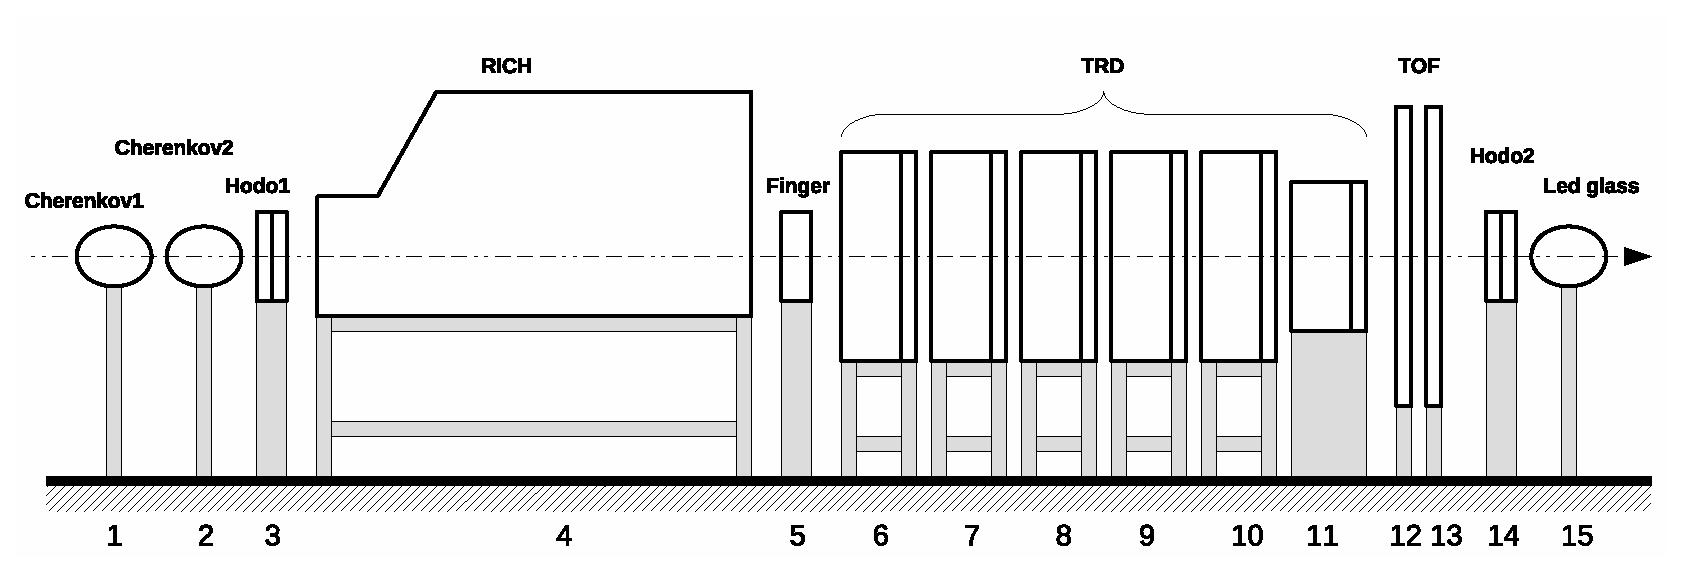
\includegraphics[width=1.0\textwidth]{pictures/Beamtime_setup_full_rev.eps}
\caption{Схема экспериментальной установки на пучковых тестах. 1,2 --- пороговые газовые Черенковские счётчики; 3,14 --- станции двухкоординатного годоскопа на основе сцинтилляционного оптического волокна; 4 --- прототип детектора Черенковских колец; 5 --- пластина из органического сцинтиллятора; 6-11 --- станции прототипа детектора переходного излучения; 12-13 --- станции прототипа время-пролётного детектора; 15 --- электромагнитный калориметр из свинцового стекла.}
\label{fig:Beamtime}
\end{figure}

Вывод пучка~T9 ускорителя PS~\cite{CERNPST9} в ЦЕРНе представляет собой смешанный вторичный пучок электронов, пионов и мюонов с импульсом, настраиваемым в диапазоне 0.5~ГэВ/c --- 10~ГэВ/c. В течение пучковых тестов пучок был настроен на импульс от~1 до~3~ГэВ/c. Длительность вывода составляла около 2~секунд, причем за это время регистрировалось в среднем 500~электронов.

Схема прототипа детектора RICH эксперимента CBM представлена на \figref{fig:Prototype}.

\begin{figure}[H]
\centering
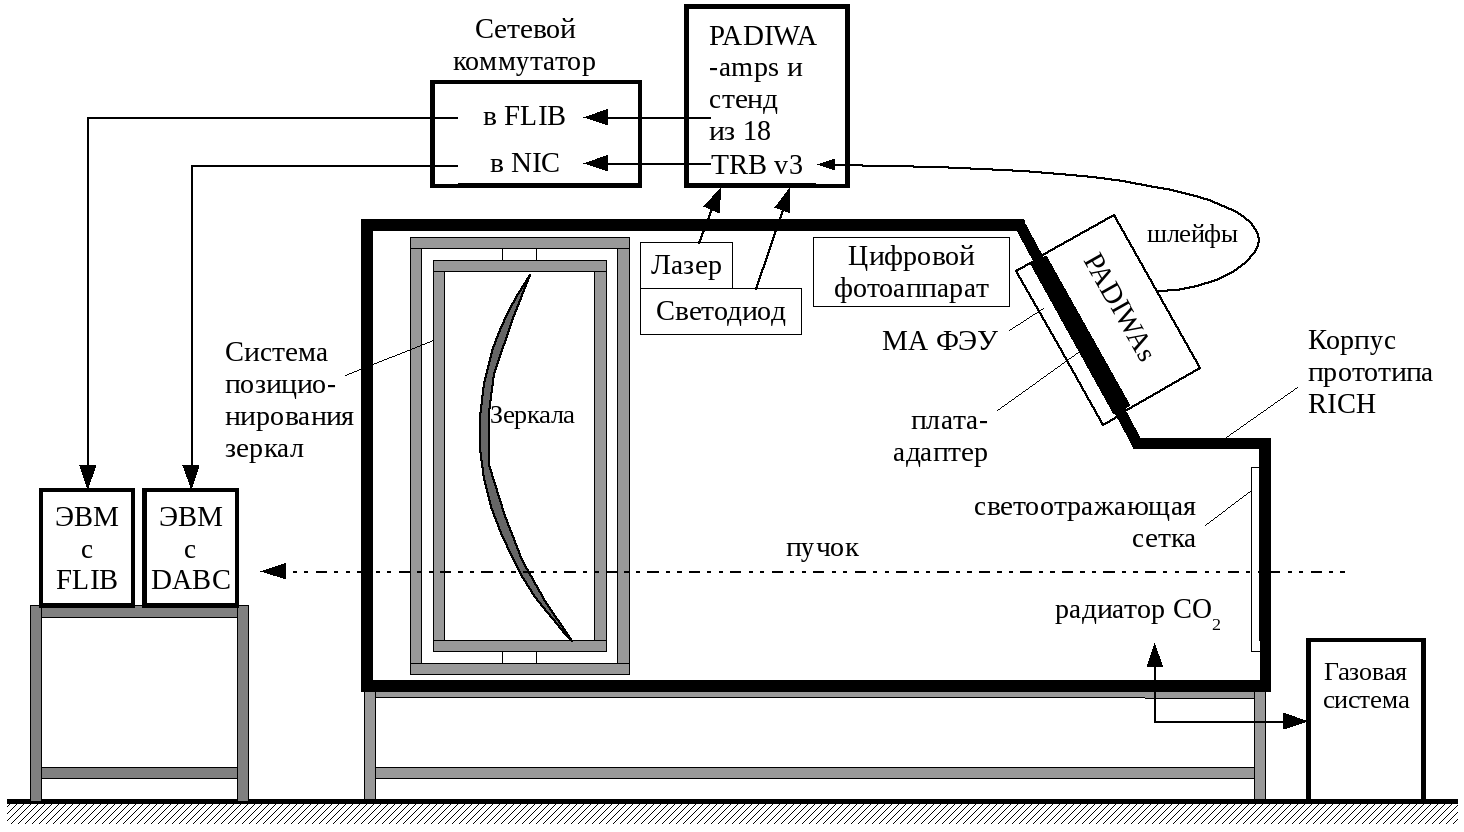
\includegraphics[width=1.0\textwidth]{pictures/10_Beamtime_setup_RICH_text.png}
\caption{Схема прототипа детектора RICH.}
\label{fig:Prototype}
\end{figure}

Габариты герметичного алюминиевого корпуса --- 1.4~м в ширину, 1.2~м в высоту и 2.4~м вдоль пучка, при этом длина пути частицы в радиаторе до зеркал --- 1.7~м. Радиатор детектора --- углекислый газ под избыточным давлением 2~мбар при комнатной температуре. Показатель преломления газа для ближнего ультрафиолета составляет при этом n=1.00045. Очистка газа и стабилизация его давления с точностью 0.1~мбар обеспечивались газовой системой, описанной в~\cite{GASSYS}. Абсолютное давление газовой смеси и температура мониторируются системой медленного управления. Актуальное значение показателя преломления автоматически вычисляется и сохраняется в данных.

Система позиционирования зеркал представляет собой раму верхнего уровня, вставляющуюся в корпус прототипа; вложенную раму, соединённую с основной рамой через два привода, обеспечивающие вращение вокруг вертикальной оси; внутреннюю раму, соединённую со вложенной рамой через два привода, обеспечивающие вращение вокруг горизонтальной оси. Сферическое зеркало радиусом кривизны 3~м состоит из 4~долей 40~см на 40~см. Каждая из долей крепится к внутренней раме через три моторизированных актуатора. Перечисленные двигатели позволяют удалённо, после установки детектора на пучке, позиционировать зеркала. Более подробно система позиционирования зеркал описана в~\cite{MIRRORMIS}.

Система диагностики положения зеркал~\cite{JORDANPR14} состоит из светоотражающей сетки, занимающей всю переднюю стенку корпуса прототипа, светодиода Roithner UVTOP240~\cite{LED} с длиной волны 245~нм и фотоаппарата, считываемого удаленно. Сетка сделана из полос ретрорефлектора шириной 10~мм и имеет прямоугольную ячейку шагом 100~мм по горизонтали и 110~мм по вертикали. Эта система позволяет контролировать точность поворота зеркал и, при наличии удалённого управления зеркалами, корректировать его. Также существуют алгоритмы расчёта поправок координат хитов для коррекции ошибок, вызванных неидеальным позиционированием зеркал. Идея метода заключается в следующем. Свет от светодиода, отражаясь от сетки и затем от зеркал, попадает в объектив фотоаппарата. На полученном кадре с помощью алгоритмов распознавания образов находятся линии сетки.
%Нафига запятая?
При наличии отклонений зеркал от идеального положения, восстановленный образ сетки будет состоять из набора отдельных отрезков.
Анализируя параметры отрезков, можно определить значения отклонений отдельных долей зеркала, значения поправок к поворотам отдельных долей зеркала, значения коррекций координат хитов.

Черенковское излучение фокусируется зеркалами на фоточувствительную камеру, содержащую матрицу 4~на~4 МА~ФЭУ, шесть из которых --- это МА~ФЭУ Hamamatsu H12700 и десять --- МА~ФЭУ Hamamatsu H8500. Данные модели МА~ФЭУ имеют сечение 52~мм на 52~мм. Часть фотоумножителей была предварительно покрыта слоем сместителя спектра толщиной 150-200~нм. В качестве сместителя спектра использовался паратерфенил ($ \approx $40\% по массе) в полимерной матрице Paraloid~B72. Сместитель спектра наносился методом погружения в раствор компонентов покрытия в дихлорметане, см.~\cite{WLSINFLUENCE}. В определённый момент во время пучковых тестов сместитель спектра был счищен. Это позволило в дальнейшем оценить влияние сместителя спектра на эффективность регистрации одиночных фотонов и на временной разброс хитов, принадлежащих одному кольцу. Для мониторирования системы считывания и калибровки относительных задержек между каналами, наряду со светодиодом, использовался лазер Alphalas Picopower LD405~\cite{ALPHALAS} с длиной волны 405~нм и длительностью импульса по паспорту менее 40~пс. Частота срабатывания лазера, так же как и светодиода, составляла 100~Гц. Интенсивность лазера была подобрана так, чтобы частота срабатывания каждого пикселя была на уровне~10\% от частоты запуска лазера.

Считывание с каждого МА~ФЭУ осуществлялось модулем, описанным в разделе~\ref{section:secModule}. Механически все 16~МА~ФЭУ монтировались на плату-адаптер, обеспечивающую герметичность корпуса и разводку высокого напряжения. Снаружи к плате-адаптеру монтировались платы предусилителей-дискриминаторов PADIWA, логический сигнал с плат PADIWA передавался по шлейфам, состоящим из витых пар и имеющих длину 2~м, к платам TRB~v3 (конфигурации~1), установленным на корпусе прототипа. Для всей камеры потребовалось всего 64~платы PADIWA и 16~плат TRB~v3 (конфигурации~1). Данные с 16~плат TRB~v3 поступали на ещё одну, 17-ю плату TRB~v3 особой конфигурации, которая помимо концентратора данных также являлась генератором и распределителем триггера считывания для всех плат TRB~v3. Импульсы с генераторов, управляющих лазером и светодиодом, а также сигналы от детекторов пучка обрабатывались платами PADIWA-amp (плата, подобная PADIWA, но позволяющая измерять амплитуду сигнала и имеющая в два раза меньшее число каналов~\cite{TRBSITE}) и оцифровывались ВЦП на ещё одной, 18-й плате TRB~v3 также нестандартной конфигурации, совмещающей ВЦП и концентратор данных. Параллельно функционировало две системы сбора данных --- одна принимала данные через стандартный сетевой интерфейс (сетевой концентратор) с каждой платы TRB~v3 по медному носителю, а другая через FLIB с одной (18-й) платы TRB~v3. Схема считывания всей камеры и детекторов пучка представлена на \figref{fig:BeamtimeReadout}. Отметим, что ЭВМ с установленной в неё платой FLIB, использовалась для приёма данных не только от прототипа RICH, но и от других детекторов.

\begin{figure}[H]
\centering
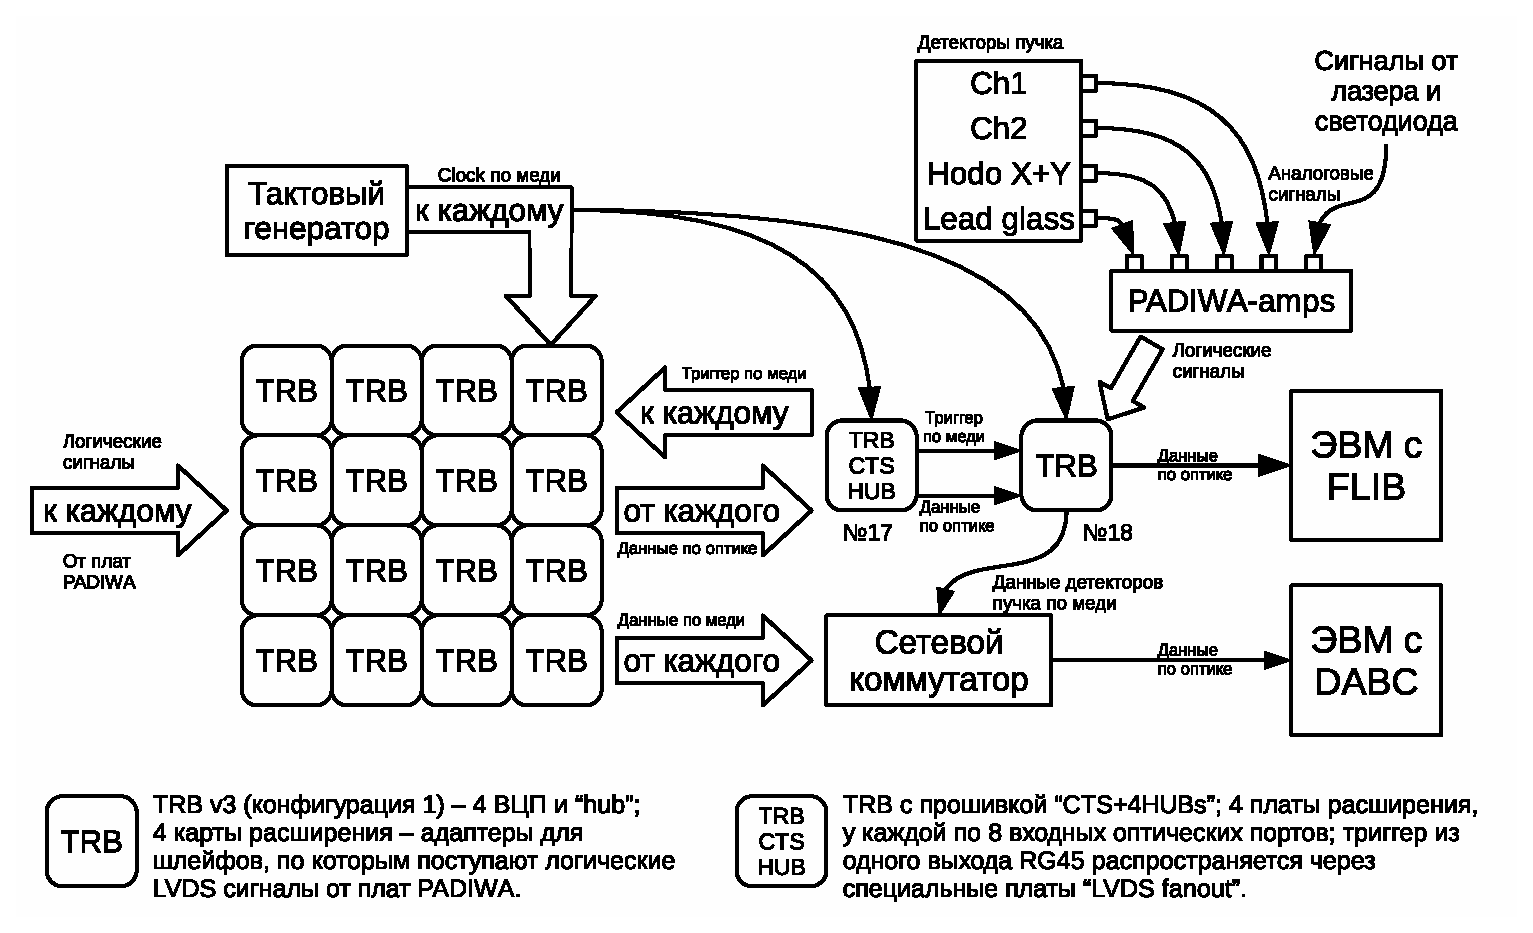
\includegraphics[width=1.0\textwidth]{pictures/11_Beamtime_readout_chain.eps}
\caption{Схема считывания всей камеры и детекторов пучка.}
\label{fig:BeamtimeReadout}
\end{figure}
